Обзор имитационной модели LTE-EPC изображен на рис. \ref{img:LTEEPC}. Состоит из двух основных компонентов:
\begin{itemize}
  \item Модель LTE. Эта модель включает LTE радио стек протоколов (RRC, PDCP, RLC, MAC, PHY). Эти объекты полностью находятся на UE и eNB узлах.
  \item Модель EPC. Эта модель включает в себя основные сетевые интерфейсы, протоколы и объекты. Эти объекты и протоколы находятся на S-GW, P-GW и MME узлах и частично на eNB узлах.
\end{itemize}

\begin{figure} [h]
  \center
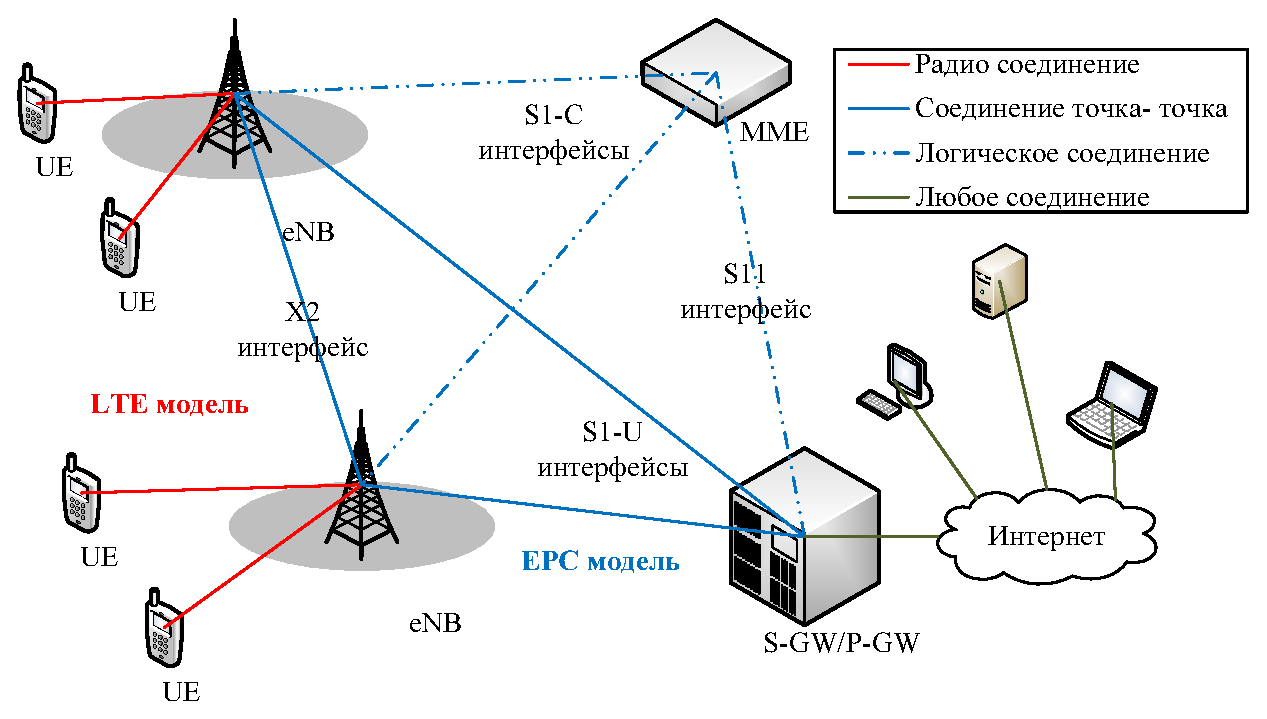
\includegraphics [width=0.95\textwidth] {LTEEPC.eps}
  \caption{Обзор имитационной модели LTE-EPC \cite{LteSimDoc}}
  \label{img:LTEEPC}
\end{figure}



\section{Архитектура LTE модели} \label{B1}
LTE модель была разработана для поддержки оценки следующих аспектов системы LTE:
\begin{itemize}
  \item Управление радио ресурсами.
  \item Пакетная обработка на основе QoS.
  \item Внутрисистемные помехи между сотами.
  \item Динамический спектральный доступ
\end{itemize}


Архитектура физического и канального уровня для модели узла UE представлена на рис. \ref{img:UEPHY} и для модели узла eNB представлена на рис \ref{img:eNBPHY}.
\begin{figure} [h]
  \center
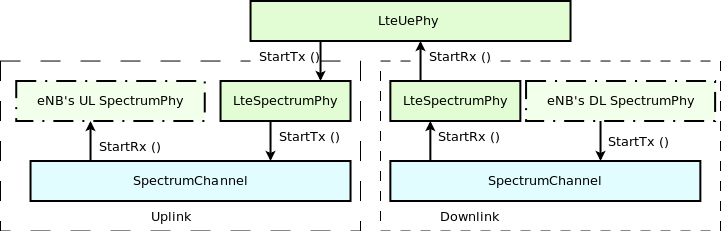
\includegraphics [width=0.95\textwidth] {UEPHY.png}
  \caption{Архитектура физического и канального уровня для модели UE \cite{LteSimDoc}}
  \label{img:UEPHY}
\end{figure}

\begin{figure} [h]
  \center
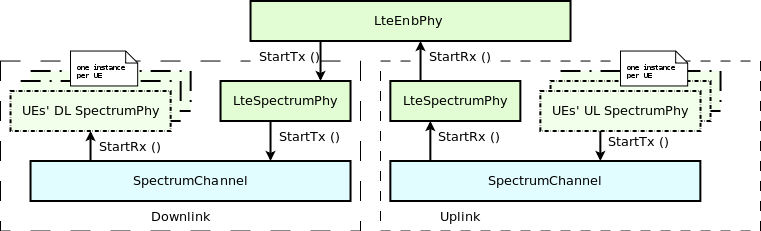
\includegraphics [width=0.95\textwidth] {eNBPHY.png}
  \caption{Архитектура физического и канального уровня для модели eNB \cite{LteSimDoc}}
  \label{img:eNBPHY}
\end{figure}

\section{Архитектура EPC модели} \label{B2}
Модели EPC обеспечивает средства для моделирования сквозного IP соединения по верх LTE модели. В частности, поддерживает соединение нескольких UE с интернетом через сеть радиодоступа с несколькими узлами eNB, подключенными к одному SGW/PGW узлу. Эта топология сети изображен на рис \ref{img:LTEEPCdata}.
Основное внимание в модели ЕРС в настоящее время сфокусировано на плоскости данных EPC. Чтобы понять архитектуру этой модели, мы сначала посмотрим на рис \ref{img:LTEEPCdata}, где представлен сквозной LTE-EPC стек протоколов таким образом каким это реализовано в симуляторе. Из рисунка видно, что самые большие упрощения введены в модели ЕРС для плоскости данных, является включение функций SGW и PGW в один узел SGW / PGW, который устраняет необходимость S5 или S8 интерфейсов, определенных в 3GPP . С другой стороны, все уровни протокола S1-U и протокола радиосвязи LTE стек, указанные в 3GPP, присутствуют.

\begin{figure} [h]
  \center
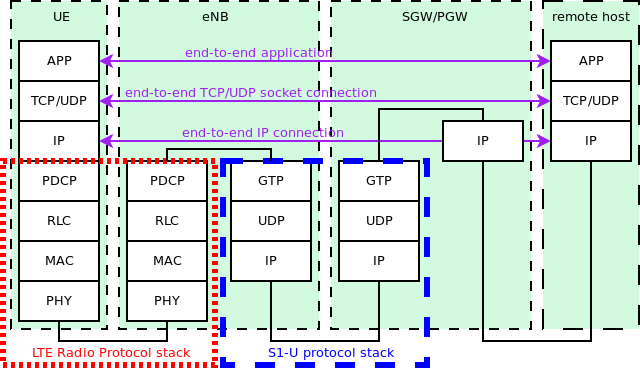
\includegraphics [width=0.95\textwidth] {LTEEPCdata.png}
  \caption{Архитектура физического и канального уровня для модели eNB \cite{LteSimDoc}}
  \label{img:LTEEPCdata}
\end{figure}

Как показано на рисунке, существует два различный уровня IP-сети. Первый это сквозной уровень, который обеспечивает сквозное подключение к пользователям; этот слой включает UE, PGW и удаленный хост (в том числе возможные интернет маршрутизаторы и хосты между ними), но не включать eNB. По умолчанию, UE присваивается публичный адрес IPv4 из 7.0.0.0/8 сети и PGW присваивается адрес 7.0.0.1, который используется всеми UE, в качестве шлюза для доступа в Интернет.
Второй слой IP сетей является ePC локальной сетью. Которая включает в себя все узлы ENB и SGW/PGW узел. Эта сеть реализован в виде набора соединений точка-точка, которые соединяют каждый eNB с SGW/PGW узлом, таким образом, SGW/PGW имеет набор устройств точка-точка, каждый из которых обеспечивает подключение к другому eNB. По умолчанию, подсети 10.xyz/30 присваивается каждому соединению точка-точка.
Как указано в 3GPP, сквозные IP соединения являются тунелями через локальную EPC IP сеть с использованием GTP/UDP/IP. Далее рассмотрим как это туннелирование реализовано в модели ЕРС. Объяснение сделано путем обсуждения сквозного потока пакетов данных.

Для начала, рассмотрим случай нисходящей линии связи, который изображен на рис \ref{img:DownloadUE}. IPv4 пакеты нисходящей линии связи генерируются от общего удаленного хоста и адресуются к одному из устройств UE. Интернет маршрутизация будет заботиться о пересылке пакета на публичный сетевой интерфейс NetDevice узла SGW/PGW, который подключен к Интернету (этот интерфейс Gi в соответствии с 3GPP терминологии). SGW/PGW имеет сетевой интерфейс VirtualNetDevice которому присваивается IP-адрес шлюза для подсети UE, следовательно, правило статической маршрутизации приведет к тому, что входящий пакет из Интернета будут проходить через VirtualNetDevice. Это сетевое устройство начинает GTP/UDP/IP туннельную процедуру, путем пересылки пакетов на выделенное приложение на узле SGW/PGW, которое называется EpcSgwPgwApplication. Это приложение выполняет следующие операции:
\begin{figure} [h]
  \center
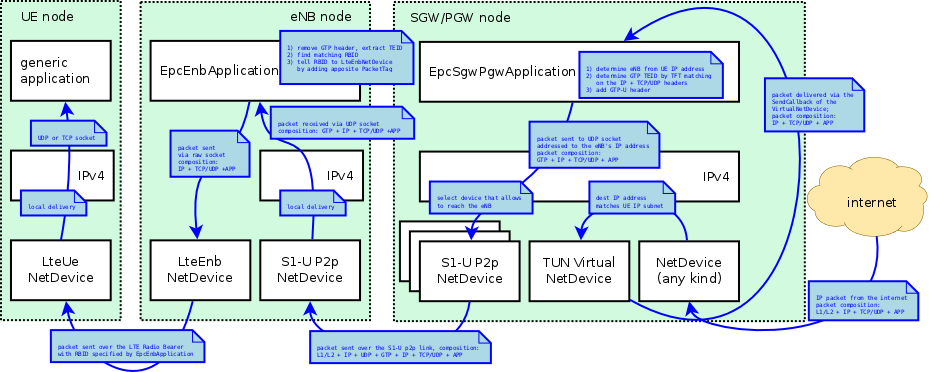
\includegraphics [width=0.95\textwidth] {DownloadUE.png}
  \caption{Поток данных нисходящей линии связи между интернетом и узлом UE \cite{LteSimDoc}}
  \label{img:DownloadUE}
\end{figure}


\begin{enumerate}
  \item Определяет eNB узел, к которому присоединен UE, смотря на IP-адрес назначения (который является адресом UE).
  \item Классифицирует пакеты, используя шаблоны транспортных потоков (TFT - Traffic Flow Templates), чтобы идентифицировать, какому ePS каналу он принадлежит. ePS каналы имеют карту соответсвия к S1-U каналам, так что эта операция возвращает идентификатор TEID (GTP-U Tunnel Endpoint Identifier), к которому принадлежит данный пакет.
  \item Добавляет соответствующие GTP-U-заголовки к пакету.
  \item Отправляет пакет через UDP-сокет к S1-U P2P NetDevice, адресуя к eNB, с которым соединен UE.
\end{enumerate}
Как следствие, пакес со сквозным IP заголовком с добавленными IP, UDP и GTP заголовками отправляется S1 соединение к eNB, где он принимается и доставляется локально (в качестве адреса назначения подставляется приватный адрес eNB). Локальный процесс доставки отправит пакет через UDP сокет к выделенному приложению EpcEnbApplication. Это приложение выполняет следующие операции:
\begin{enumerate}
  \item Удаляет заголовок GTP и извлекает TEID, который содержится в нем.
  \item Используя на взаимно-однозначное соответствие между S1-U каналами и радио каналами (который является 3GPP требованием), определяет идентификатор радиоканала (RBID -Radio Bearer ID), к которому принадлежит данный пакет.
  \item Записывает RBID в выделенном тег под названием LteRadioBearerTag, который добавляется к пакету.
  \item Пересылает пакет к приложению LteEnbNetDevice eNB узла через raw сокет.
\end{enumerate}
Следует отметить, что в этот момент, внешним заголовком пакета является сквозной IP заголовок, поскольку IP/UDP/GTP заголовки S1 стека протоколов уже были удалены. После приема пакета от EpcEnbApplication, LteEnbNetDevice будет извлекать RBID из LteRadioBearerTag, и на основе RBID определит экземпляр радиоканала (и соответствующие PDCP и RLC экземпляры протокола), которые затем используются для передачи пакета к UE через радиоинтерфейс LTE. В конце, приложение LteUeNetDevice узла UE получит пакет и доставит его локально через IP стек протоколов, которые в свою очередь доставит его к приложению на узле UE, которое является конечной точкой нисходящей линии связи.

В случае восходящего соединения, показанном на рис. \ref{img:UploadUE} , IP пакеты создаются приложением внутри UE, и передается локальным стеком протоколов TCP / IP к приложению LteUeNetDevice узла UE. LteUeNetDevice затем выполняет следующие операции:
\begin{enumerate}
  \item Классифицирует пакет, испоьзуя TFT, и определяет радиоканал, к которому принадлежит пакет (и соответствующие RBID).
  \item Определяет соответствующий экземпляр протокола PDCP, который является точкой входа LTE радио стеком протоколов для этого пакета.
  \item Посылает пакет к eNB через LTE радио стек протоколов.
\end{enumerate}
eNB принимает пакет через его сетевой интерфейс LteEnbNetDevice. Поскольку существует один экземпляр протокола PDCP и RLC для каждого радиоканала, LteEnbNetDevice способен определить RBID пакета. Это RBID затем записывается в LteRadioBearerTag, который добавляется к пакету. LteEnbNetDevice затем пересылает пакет EpcEnbApplication через сокет пакета.
При получении пакета EpcEnbApplication выполняет следующие операции:
\begin{enumerate}
  \item Извлекает RBID из тега LteRadioBearerTag в пакете.
  \item Определяет соответствующий EPS канал и GTP-U TEID за счет использования на взаимно-однозначное соответствие между S1-U каналами и радиоканалами.
  \item Добавляет GTP-U заголовок пакета, в том числе TEID, который был определен ранее.
  \item Посылает пакет на SGW/PGW узел через UDP сокет подключенный к S1-U сетевому точка-точка устройству.
\end{enumerate}

В этот момент пакет содержит S1-U IP, UDP и GTP заголовки в дополнение к первоначальному сквозному IP заголовку. Когда пакет поступает на соответствующий S1-U P2P NetDevice на узле SGW/PGW, он доставляется локально. Локальный процесс доставки направляет пакет к EpcSgwPgwApplication через соответствующий UDP сокет. EpcSgwPgwApplication затем удаляет заголовок GTP и пересылает пакет VirtualNetDevice. На данный момент, внешним заголовком пакета является сквозной IP заголовок. Следовательно, если адрес назначения в этот заголовке является удаленным узлом в интернете, пакет отправляется в интернет через соответствующие сетевое устройство NetDevice на узле SGW/PGW. В случае, если пакет адресован другому UE, IP стек SGW/PGW перенаправит пакет снова к сетевому устройству VirtualNetDevice, и пакет будет проходить через процесс доставки через нисходящее соединение для того, чтобы достичь пункта назначения UE.

\begin{figure} [h]
  \center
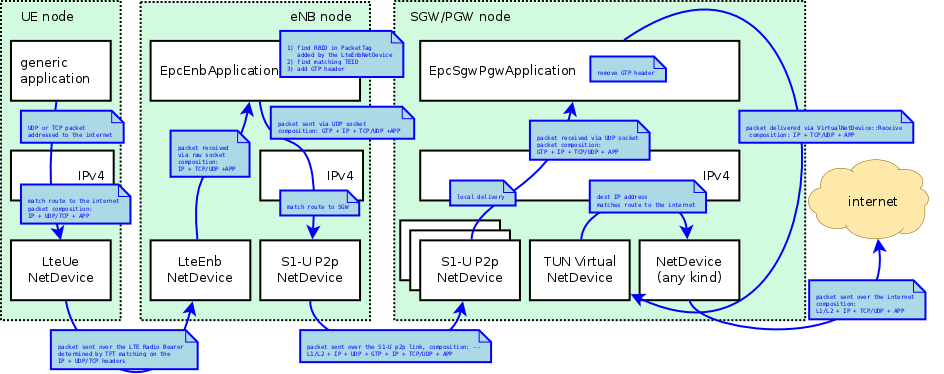
\includegraphics [width=0.95\textwidth] {UploadUE.png}
  \caption{Поток данных восходящей линии связи между узлом UE и интернетом \cite{LteSimDoc}}
  \label{img:UploadUE}
\end{figure}



